% Options for packages loaded elsewhere
\PassOptionsToPackage{unicode}{hyperref}
\PassOptionsToPackage{hyphens}{url}
\documentclass[
]{article}
\usepackage{xcolor}
\usepackage{amsmath,amssymb}
\setcounter{secnumdepth}{-\maxdimen} % remove section numbering
\usepackage{iftex}
\ifPDFTeX
  \usepackage[T1]{fontenc}
  \usepackage[utf8]{inputenc}
  \usepackage{textcomp} % provide euro and other symbols
\else % if luatex or xetex
  \usepackage{unicode-math} % this also loads fontspec
  \defaultfontfeatures{Scale=MatchLowercase}
  \defaultfontfeatures[\rmfamily]{Ligatures=TeX,Scale=1}
\fi
\usepackage{lmodern}
\ifPDFTeX\else
  % xetex/luatex font selection
\fi
% Use upquote if available, for straight quotes in verbatim environments
\IfFileExists{upquote.sty}{\usepackage{upquote}}{}
\IfFileExists{microtype.sty}{% use microtype if available
  \usepackage[]{microtype}
  \UseMicrotypeSet[protrusion]{basicmath} % disable protrusion for tt fonts
}{}
\makeatletter
\@ifundefined{KOMAClassName}{% if non-KOMA class
  \IfFileExists{parskip.sty}{%
    \usepackage{parskip}
  }{% else
    \setlength{\parindent}{0pt}
    \setlength{\parskip}{6pt plus 2pt minus 1pt}}
}{% if KOMA class
  \KOMAoptions{parskip=half}}
\makeatother
\usepackage{graphicx}
\makeatletter
\newsavebox\pandoc@box
\newcommand*\pandocbounded[1]{% scales image to fit in text height/width
  \sbox\pandoc@box{#1}%
  \Gscale@div\@tempa{\textheight}{\dimexpr\ht\pandoc@box+\dp\pandoc@box\relax}%
  \Gscale@div\@tempb{\linewidth}{\wd\pandoc@box}%
  \ifdim\@tempb\p@<\@tempa\p@\let\@tempa\@tempb\fi% select the smaller of both
  \ifdim\@tempa\p@<\p@\scalebox{\@tempa}{\usebox\pandoc@box}%
  \else\usebox{\pandoc@box}%
  \fi%
}
% Set default figure placement to htbp
\def\fps@figure{htbp}
\makeatother
\setlength{\emergencystretch}{3em} % prevent overfull lines
\providecommand{\tightlist}{%
  \setlength{\itemsep}{0pt}\setlength{\parskip}{0pt}}
\usepackage{bookmark}
\usepackage[authoryear,round]{natbib}
\IfFileExists{xurl.sty}{\usepackage{xurl}}{} % add URL line breaks if available
\urlstyle{same}
\hypersetup{
  pdftitle={Does the Bond Market Need a Bank Account?},
  pdfauthor={Shaohui Wang},
  hidelinks,
  pdfcreator={LaTeX via pandoc}}

\title{Does the Bond Market Need a Bank Account?}
\usepackage{etoolbox}
\makeatletter
\providecommand{\subtitle}[1]{% add subtitle to \maketitle
  \apptocmd{\@title}{\par {\large #1 \par}}{}{}
}
\makeatother
\subtitle{Forward Measure Consistency and Interest Rate Pricing}
\author{Shaohui Wang\footnote{shaohui.wang@hotmail.com}}
\date{July 2026}

\begin{document}
\maketitle

\section{Abstract}\label{abstract}

The standard no-arbitrage framework for bond markets assumes the
existence of a tradable bank account \(B(t)\) as universal numéraire.
But \(B\) is not directly traded --- it must be synthesized from
zero-coupon bonds via a rolling strategy that, in continuous time,
requires rebalancing through uncountably many maturities. Meanwhile,
practitioners price and hedge using T-forward measures \(Q^T\), each
derived from a single tradable bond, without invoking \(B\) at all.

This raises a question: does the family \(\{Q^T\}\) of local pricing
measures, built from tradable bonds alone, necessarily assemble into a
single global measure \(Q\) --- or is \(Q\) (and therefore \(B\)) an
additional assumption?

We formalize this question and show it has substance. In discrete time
the answer is yes: a consistent family of forward measures always
exists, and the bank account emerges as a self-financing rolling
strategy via a four-way FTAP equivalence. In continuous time, we provide
a precise, \(Q\)-free definition of forward-measure consistency
(Definition 3.2.1), under which the pairwise conditions provably
self-propagate (Lemma 2.4.1), with bond-ratio bubbles excluded by
hypothesis. The obstruction to a global \(Q\) is therefore neither
incompatibility of the measure family nor a projective-limit extension
problem: it is the construction of the numéraire \(B\) itself. We state
the resulting existence question in a falsifiable form and leave it
open.

To demonstrate that the question is not vacuous, we conduct a
descriptive empirical exercise: independent calibration of Gaussian HJM
models on different maturity segments of the EUR government bond market.
The implied market prices of risk differ systematically across segments,
in a divergent pattern that the synthetic controls we examined do not
replicate. This does not answer the question --- the observed pattern is
consistent with either absence of a single \(Q\) or the inadequacy of
the model class used --- but it establishes that the question has
empirical content.

\section{1. Introduction}\label{introduction}

\subsection{1.1 The Question}\label{the-question}

The foundational insight of \citet{BlackScholes1973} and \citet{Merton1973}
is that derivative prices are determined by replication using tradable
assets. The risk-neutral measure \(Q\), introduced by \citet{HarrisonKreps1979}, encodes this replication logic mathematically \citep{BinghamKiesel2004}.

In bond markets, the tradable assets are zero-coupon bonds
\(p(\cdot,T)\). The bank account
\(B(t) = \exp\left( \int_{0}^{t} r(s) \, ds \right)\) --- the standard
numéraire of the FTAP --- is not directly traded. To construct it, one
must execute a rolling strategy: hold the just-maturing bond, roll the
proceeds into the next. In discrete time, this is a finite,
self-financing strategy using traded bonds. In continuous time, it
requires continuous rebalancing through an uncountable family of
maturities --- and the convergence of this strategy is not guaranteed by
the well-behavedness of individual bond prices.

Practitioners already work without \(B\): to price a caplet at \(T\),
they use the T-bond as numéraire and \(Q^T\) as pricing measure. Each
operation is faithful to the Black-Scholes-Merton logic --- replicate
using tradable instruments, extract the price. This paper takes the
practitioners' approach seriously and asks:

\begin{quote}
\emph{Does the family \(\{Q^T\}\) of local pricing measures, derived
from tradable bonds, necessarily cohere into a single global measure
\(Q\)?}
\end{quote}

If yes, the bank account is a derived object --- it emerges from the
consistency of local pricing, and the standard FTAP is confirmed from
the bottom up. If no, the standard theory requires an assumption (the
existence of \(Q\) and \(B\)) that goes beyond what tradable instruments
can deliver.

In discrete time, we show the answer is yes: a consistent family always
exists and \(B\) is constructible (Section 2). In continuous time, we
formalize the question precisely, locate the obstruction in the
construction of the numéraire \(B\), and leave it open (Section 3). We
then present a descriptive empirical exercise showing the question has
empirical content (Section 4).

To be clear about what is and is not established: we contribute (i) a
precise, \(Q\)-free definition of forward-measure consistency
(Definition 3.2.1), under which the pairwise conditions provably
self-propagate (Lemma 2.4.1), with bond-ratio bubbles excluded by
hypothesis; (ii) the identification of the numéraire \(B\) --- not
measure incompatibility, and not a projective-limit problem --- as the
sole locus of the continuous-time obstruction (Section 3.4); and (iii) a
descriptive demonstration that the question has empirical content
(Section 4). We do not resolve the continuous-time existence question,
and we do not claim a relationship to existing large-market results
beyond a precise statement of the residual gap (Section 5).

\subsection{1.2 Related Work}\label{related-work}

\citet{MusielaRutkowski1997} and \citet{DoberleinSchweizerStricker2000} proved uniqueness of the implied savings account --- but took
existence as given. Our question is the complement: existence given
local data.

The closest existing work is \citet{KleinSchmidtTeichmann2016}, who
investigate bond markets where ``the bank account process is not a valid
numéraire or does not exist at all.'' They argue this is ``not the
exception but rather the rule'' when starting from terminal bonds as
numéraires. Using large financial market methods, they prove that no
asymptotic free lunch (NAFL) is equivalent to the existence of an
equivalent local martingale measure with respect to a terminal bond, and
they construct a generalized bank account as a limit of convex
combinations of roll-over bonds. Their work establishes the theoretical
framework for bond markets without a classical bank account. Our
question starts from a different point --- pairwise measure consistency
(Definition 3.2.1) rather than a no-arbitrage condition on trading
strategies --- and the relationship between these two starting points
is, to our knowledge, not established. \citeauthor{KleinSchmidtTeichmann2016}'s
generalized bank account is a limit object that may differ from the
classical \(B\); whether pairwise consistency of \(\{Q^T\}\) implies
NAFL (or vice versa) is an open question that connects our work to
theirs; Section 5 states the residual gap precisely.

\citet{Herdegen2017} develops a numéraire-independent FTAP for general
markets. Whether his condition \(\text{NA}^{\text{ni}}\) coincides with,
is weaker than, or is stronger than our Bond-Family condition (BF) in
continuous-time bond markets is, to our knowledge, open.

A continuous-time bond market with a continuum of maturities is a large
financial market in the sense of \citet{CuchieroKleinTeichmann2016},
\citet{DeDonno2004}, \citet{TakokaSchweizer2014}, and \citet{CarmonaTehranchi2006}. Our question --- does \(\{Q^T\}\) cohere into a single \(Q\)?
--- is related to the existence of an equivalent martingale measure in
such markets. We note the connection but do not pursue it formally; the
bond-specific structure may give the question a different character from
the general large-market problem, though we cannot establish this
precisely.

\citet{Filipovic2001,Filipovic2009} studies consistency problems for HJM models ---
when HJM dynamics preserve the shape of the yield curve within a given
parametric family. This is a related but distinct question: Filipović
asks whether a model is internally consistent with a family of initial
curves, while we ask whether independently calibrated local measures are
mutually consistent. The tools developed in \citeauthor{Filipovic2001}'s framework
(function spaces, regularity conditions) may be relevant to resolving
our question, but we do not establish the connection formally.

\citet{Henrard2007} and \citet{Morini2009} identified the post-2007 failure of
single-curve pricing. The multi-curve literature \citep{FilipovicTrolle2013,Crepey2015,GrbacRunggaldier2015} addresses a
different mechanism --- counterparty credit risk in interbank rates ---
but the conceptual parallel is suggestive: the single-curve assumption
is the assumption that \(\{Q^T\}\) coheres.

In retrospect, our question belongs to what has been called the
bottom-up or model-free tradition in mathematical finance: Samuelson
(1938) asked whether observed choices imply preferences exist; \citet{Hobson1998} and the model-free finance programme \citep{DavisHobson2007,Acciaio2013} ask what can be inferred from observed prices
without assuming a model; \citet{BalbasIbanezLopez2002} use
projective limits of measure families to characterize no-arbitrage over
infinite horizons. We recognized this connection during the development
of the paper, not at the outset.

\subsection{1.3 Structure}\label{structure}

Section 2 establishes the proof of concept: in discrete time, a
consistent family of forward measures always exists and glues into a
global \((Q, B)\). Section 3 formalizes the continuous-time question and
locates the obstruction in the numéraire. Section 4 presents a
descriptive empirical exercise demonstrating the question has empirical
content. Section 5 identifies directions for future investigation.

\section{2. Discrete Time: Proof of
Concept}\label{discrete-time-proof-of-concept}

\subsection{2.1 Setup}\label{setup}

Let
\((\Omega, \mathcal{F}, (\mathcal{F}_t)_{t=0,\ldots,N}, \mathbb{P})\) be
a filtered probability space. The market consists of default-free
zero-coupon bonds \(p(t,T)\) with \(p(T,T) = 1\) and \(p(t,T) > 0\),
plus risky assets \(X^1,\ldots,X^d\). No bank account is assumed.

A trading strategy is a predictable process specifying holdings in each
asset. It is self-financing if portfolio value changes arise solely from
price movements. An arbitrage is a zero-cost self-financing strategy
producing \(V_N \geq 0\) a.s. with \(\mathbb{P}(V_N > 0) > 0\).

\subsection{2.2 The Rolling Bond
Strategy}\label{the-rolling-bond-strategy}

\textbf{Proposition 2.2.1.} Define \(B(0) := 1\) and
\(B(t) := \prod_{s=1}^{t} 1/p(s-1,s)\). Then \(B\) is the value process
of a self-financing strategy holding, during each period \((t-1,t]\),
exactly \(B(t-1)/p(t-1,t)\) units of the just-maturing bond
\(p(\cdot,t)\). The one-period return \(1/p(t-1,t)\) is deterministic
given \(\mathcal{F}_{t-1}\).

\subsection{2.3 The Four Equivalences}\label{the-four-equivalences}

\textbf{Proposition 2.3.1 (Bond-Based FTAP, Discrete Time).} The
following are equivalent:

\textbf{(NA)} No arbitrage exists in the bond market.

\textbf{(EMM)} \(\exists Q \sim P\) such that \(S(t)/B(t)\) is a
\(Q\)-martingale for all traded assets \(S\).

\textbf{(RF)} \(\exists Q \sim P\) such that
\(E^Q[R_t^S \mid \mathcal{F}_{t-1}]\) equals the just-maturing bond
return \([1 - p(t-1,t)]/p(t-1,t)\) for all traded \(S\), where
\(R_t^S := S(t)/S(t-1) - 1\) is the one-period simple return.

\textbf{(BF)} For each \(T \in \{1,\ldots,N\}\), \(\exists Q^T \sim P\)
such that \(S(t)/p(t,T)\) is a \(Q^T\)-martingale for all traded assets
\(S\) and \(t \le T\).

Moreover, the forward measures constructed in the proof of
\((\text{EMM}) \Rightarrow (\text{BF})\) satisfy the consistency
relation

\[\frac{dQ^{T_1}}{dQ^{T_2}}\bigg|_{\mathcal{F}_{T_1}} = \frac{p(0,T_2)}{p(0,T_1) \cdot p(T_1,T_2)}   \quad (2.1)\]

involving only bond prices, with no reference to \(B\).

\emph{Proof sketch.} \((\text{NA}) \iff (\text{EMM})\): Rolling
construction makes \(B\) tradable; \citet{HarrisonPliska1981} applies.
\((\text{EMM}) \iff (\text{RF})\): Algebraic reformulation --- the
equivalence follows from multiplying both sides of the martingale
condition by \(B(t-1)/S(t-1)\) and using \(B(t)/B(t-1) = 1/p(t-1,t)\).
\((\text{EMM}) \Rightarrow (\text{BF})\): Bayes' formula with density
\(Z^T_t := p(t,T)/[B(t) \cdot p(0,T)]\).
\((\text{BF}) \Rightarrow (\text{NA})\): Under \(Q^N\),
\(V^\varphi_t/p(t,N)\) is a martingale; \(V_0 = 0\) forces \(V_N = 0\)
a.s. Full proofs in Appendix A. \(\quad\square\)

\textbf{Remark.} The proposition assembles standard ingredients
(\citeauthor{HarrisonPliska1981} for \((\text{NA}) \iff (\text{EMM})\), Bayes' formula
for the numéraire change, \citealt{GemanElKarouiRochet1995} for the general
framework). Its purpose here is not mathematical novelty but to
establish the four-way equivalence and to identify the precise point
where the argument uses discreteness: the chain rule across maturity
triples is a finite number of conditions. This is the point that becomes
problematic in continuous time.

\subsection{2.4 A Consistent Family Always Exists --- But Only in
Discrete
Time}\label{a-consistent-family-always-exists-but-only-in-discrete-time}

Given (EMM), the family \(\{Q^T\}\) constructed via
\(Z^T_t = p(t,T)/[B(t) \cdot p(0,T)]\) satisfies (2.1), and the chain
rule
\[\frac{dQ^{T_1}}{dQ^{T_3}} = \frac{dQ^{T_1}}{dQ^{T_2}} \cdot \frac{dQ^{T_2}}{dQ^{T_3}}\]
across maturity triples is a finite number of conditions, each satisfied
by construction. In an incomplete market other forward-measure
selections exist; (2.1) singles out the mutually compatible family.

The discreteness that does the work here is discreteness of
\emph{trading}: \(B\) is a finite product of one-period bond returns.
With finitely many maturities but continuous trading, \(B\) still need
not exist for all \(t\) (Section 3.4). That a consistent family glues
into a global \((Q, B)\) is, under discrete trading, a consequence of
finitude, not of structure.

\textbf{Lemma 2.4.1 (Pairwise consistency is self-propagating).}
\emph{Under the true-martingale hypothesis of Definition 3.2.1, if a
family \(\{Q^T\}\) satisfies (3.1) for every pair, it satisfies the
triple relation automatically: for \(T_1 < T_2 < T_3\),}
\[\frac{dQ^{T_1}}{dQ^{T_3}}\bigg|_{\mathcal{F}_{T_1}} = \frac{dQ^{T_1}}{dQ^{T_2}}\bigg|_{\mathcal{F}_{T_1}} \cdot \frac{dQ^{T_2}}{dQ^{T_3}}\bigg|_{\mathcal{F}_{T_1}}.\]

\emph{Proof.} By the true-martingale hypothesis, the bond ratio
\(p(\cdot,T_2)/p(\cdot,T_3)\) is a true \(Q^{T_3}\)-martingale on
\([0,T_2]\), so optional sampling at \(t = T_1\) is valid and (3.1) for
the pair \((T_2, T_3)\) gives
\(\frac{dQ^{T_2}}{dQ^{T_3}}\big|_{\mathcal{F}_{T_1}}
= \frac{p(0,T_3)}{p(0,T_2)} \cdot \frac{p(T_1,T_2)}{p(T_1,T_3)}\).
Multiplying by (3.1) for \((T_1, T_2)\) and cancelling \(p(T_1,T_2)\)
and \(p(0,T_2)\) returns (3.1) for \((T_1, T_3)\). \(\square\)

The cocycle is therefore not an additional requirement: pairwise
consistency is never the source of failure. Whatever obstructs the
passage to a global \(Q\) in continuous time, it is not incompatibility
of the measure family at any finite level.

\textbf{Remark (Relationship to Herdegen 2017).} In bond markets with
strictly positive prices, \citeauthor{Herdegen2017}'s numéraire-independent no-arbitrage
(\(\text{NA}^{\text{ni}}\)) coincides with NA in discrete time: with
finitely many assets all having strictly positive prices, any numéraire
is equivalent to any other, and the no-arbitrage conditions coincide
(Herdegen 2017). Our Bond-Family formulation (BF) is the only condition
among the four equivalences that extends to continuous time without
assuming \(B\). Whether (BF) in continuous time is equivalent to, weaker
than, or stronger than \(\text{NA}^{\text{ni}}\) restricted to bond
markets is an open question.

\section{3. Continuous Time: The
Question}\label{continuous-time-the-question}

\subsection{3.1 Where the Proof Breaks}\label{where-the-proof-breaks}

In continuous time, the rolling strategy requires trading at every
instant through uncountably many bonds (cf.~\citealt{Bjork1997}, \citealt{DoberleinSchweizer2001}). The Bond-Family condition survives --- each \(Q^T\)
uses only the tradable T-bond --- but consistency over a continuum of
maturities is no longer automatic.

\subsection{3.2 Forward-Measure
Consistency}\label{forward-measure-consistency}

We define the key concept without presupposing \(Q\) or \(B\).

\textbf{Definition 3.2.1 (Forward-Measure Consistency).} Let
\(\{Q^T\}_{T \in \mathcal{T}}\) be a family of probability measures on
\((\Omega, \mathcal{F})\), each equivalent to \(\mathbb{P}\), indexed by
a set of maturities \(\mathcal{T} \subseteq [0, T^*]\). Assume that for
each \(T\), \(S(t)/p(t,T)\) is a \(Q^T\)-local martingale on \([0,T]\)
for all traded assets \(S\), including bonds of all maturities (the
forward martingale property; for a bond \(p(\cdot,T')\) with \(T' < T\),
the requirement is on \([0, T' \wedge T]\)), and that for each pair
\(T_1 < T_2\) the bond ratio \(p(\cdot,T_1)/p(\cdot,T_2)\) is a
\emph{true} \(Q^{T_2}\)-martingale on \([0,T_1]\) --- equivalently, no
bond-ratio bubble arises up to the shorter maturity. The family is
\emph{consistent} if for all \(T_1 < T_2\) in \(\mathcal{T}\):

\[\frac{dQ^{T_1}}{dQ^{T_2}}\bigg|_{\mathcal{F}_{T_1}} = \frac{p(0,T_2)}{p(0,T_1) \cdot p(T_1,T_2)}.   \quad (3.1)\]

A remark on the status of (3.1). It is a genuine condition, not a
consequence of the bare forward martingale property. Under \(Q^{T_2}\),
the change of numéraire from the \(T_2\)-bond to the \(T_1\)-bond
produces \emph{a} measure with density (3.1) --- a valid \(T_1\)-forward
measure. But in an incomplete market forward measures are not unique,
and the family member \(Q^{T_1}\) need not coincide with this
numéraire-change image. Consistency is precisely the requirement that
the family's selections are mutually compatible. Note that the
true-martingale clause in the definition's standing assumption is
exactly what makes the right-hand side of (3.1) a bona fide
Radon-Nikodym density: for the pair \((T_1,T_2)\) the bond ratio
\(p(\cdot,T_1)/p(\cdot,T_2)\) is a non-negative \(Q^{T_2}\)-local
martingale with terminal value \(1/p(T_1,T_2)\), hence a
supermartingale, and its expectation equals \(p(0,T_1)/p(0,T_2)\) --- so
(3.1) integrates to one --- if and only if it is a true martingale
rather than a strict local one. A strict local martingale (a bond-ratio
bubble) would make the right-hand side integrate to less than one. The
definition therefore \emph{presupposes} the absence of bond-ratio
bubbles up to each shorter maturity; it does not derive it. (On
strict-local- martingale bubbles and their characterisation via change
of numéraire, see Cox and Hobson 2005, Jarrow, Protter, and Shimbo 2010,
and Protter 2013.)

\textbf{Remark.} When \(\mathcal{T}\) is finite, condition (3.1)
suffices: Proposition 2.3.1 constructs \(Q\) and \(B\) from the family.
By Lemma 2.4.1 the pairwise conditions are mutually compatible at every
finite level even when \(\mathcal{T}\) is a continuum --- so the
obstruction to a global \(Q\), if any, is \emph{not} incompatibility of
the measure family, nor a projective-limit extension problem (every
\(Q^T\) already lives on the same \((\Omega, \mathcal{F})\); nothing
must be extended to a limit space). What a global risk-neutral measure
requires beyond the family is a \emph{numéraire process} \(B\): a single
\(Q \sim \mathbb{P}\) and a strictly positive adapted \(B\) with
\(\frac{dQ^T}{dQ}\big|_{\mathcal{F}_t} = \frac{p(t,T)}{B(t) p(0,T)}\)
for every \(T\). The risk-neutral measure is not any single \(Q^T\); it
is anchored by \(B\). Identifying when such a \(B\) can be constructed
is, to our understanding, the core of the continuous-time problem.

\textbf{Why standard extension theorems do not immediately apply.} A
natural reaction is that the Kolmogorov extension theorem (or its
measure-theoretic variants) should resolve the question: given a
consistent family of finite-dimensional distributions, the theorem
constructs a measure on the projective limit. However, the pairwise
consistency condition (3.1) is not of Kolmogorov type. Kolmogorov
consistency relates measures on \emph{nested sub-$\sigma$-algebras} via
restriction: \(\mu_{n+1}|_{\mathcal{F}_n} = \mu_n\). Our condition (3.1)
relates measures on the \emph{same} $\sigma$-algebra \(\mathcal{F}\) via
Radon-Nikodym derivatives determined by bond prices. These are
structurally different: (3.1) specifies how the measures \emph{reweight}
each other, not how they \emph{restrict}. The passage from pairwise
reweighting to a global measure requires constructing a process \(B\)
such that each \(Q^T\) arises as a change of numéraire from \(Q\) --- a
stronger condition than mere compatibility of restrictions. We do not
know whether existing projective limit frameworks (such as \citealt{BalbasIbanezLopez2002}) can be adapted to this setting.

\subsection{3.3 The Question, Precisely
Stated}\label{the-question-precisely-stated}

The question of this paper:

\begin{quote}
\emph{Given a family \(\{Q^T\}_{T \in [0,T^*]}\) satisfying Definition
3.2.1, does there exist a probability measure \(Q \sim \mathbb{P}\) and
a strictly positive adapted process \(B\) such that \(S(t)/B(t)\) is a
\(Q\)-local martingale for all traded assets, each deflated bond
\(p(\cdot,T)/B\) is a }true* \(Q\)-martingale, and each \(Q^T\)
coincides on \(\mathcal{F}_T\) with the T-forward measure induced by
\(Q\)?*
\end{quote}

The true-martingale requirement on deflated bonds mirrors the standing
assumption of Definition 3.2.1: it is what makes each induced density
\(Z^T_t = p(t,T)/[B(t)\,p(0,T)]\) a bona fide Radon-Nikodym derivative,
so that the induced forward measures are well-defined.

In discrete time the answer is yes (Section 2). In continuous time it
is, to our knowledge, open.

We note that in the standard HJM framework driven by finite-dimensional
Brownian motion, the existence of \(Q\) is equivalent to the HJM drift
condition
\(\alpha(t,T) = \sigma(t,T) \cdot \int_t^T \sigma(t,s) \, ds\). The
``if'' direction is textbook (\citealt{HeathJarrowMorton1992}). Whether
forward-measure consistency \emph{forces} the drift condition --- the
``only if'' direction --- is the non-trivial question. We state this as
an open problem, not a hypothesis we are in a position to resolve. The
restriction to finite-dimensional driving noise is substantive; under
infinite-dimensional noise (cylindrical Brownian motion), the question
may take a different form.

\subsection{\texorpdfstring{3.4 Where the Obstruction Lives: the
Numéraire
\(B\)}{3.4 Where the Obstruction Lives: the Numéraire B}}\label{where-the-obstruction-lives-the-numuxe9raire-b}

By Lemma 2.4.1 the measure family is internally consistent at every
finite level, so the continuous-time question reduces to a single
object: can the numéraire \(B\) be constructed? Two features make this
non-automatic, and both are about \emph{continuous trading}, not about
the cardinality of the maturity set.

First, \(B(t) = \exp\left(\int_0^t r(s)\, ds\right)\) requires the short
rate \(r(s) = f(s,s)\) at every instant. The discrete-time rolling
strategy (Proposition 2.2.1) builds \(B\) as a finite product of
just-maturing bond returns; in continuous time it becomes a continuously
rebalanced strategy whose convergence is not guaranteed by the
well-behavedness of individual bonds. This is a
continuous-\emph{trading} phenomenon: even with finitely many
maturities, \(B\) need not be constructible for all \(t\).

Second, \(r(s) = f(s,s)\) is the diagonal restriction of the forward
surface \(f(s,T)\). A pointwise diagonal evaluation requires more
regularity than the integrated quantities
\(p(t,T) = \exp(-\int_t^T f(t,u)\,du)\) that the market actually quotes.
We note this as a \emph{heuristic analogy} with the trace problem in
functional analysis (where restricting a function to a lower-dimensional
set requires Sobolev regularity above a threshold), not as an
established mechanism: the regularity in question is that of the
\emph{joint} surface near the diagonal \(T = t\), and we are aware of no
evidence that EUR forward surfaces are irregular in this sense ---
indeed their evident smoothness in the maturity direction (which is what
makes parametric fits such as Svensson viable) cuts the other way. We
stress, however, that the relevant regularity is the \emph{joint}
behaviour of \((s,T) \mapsto f(s,T)\) as \(T \to s\) --- the
diagonal-approach regularity --- which is not the same as marginal
smoothness in \(T\) at fixed \(s\); smoothness of each maturity slice
does not by itself control how the slices behave in the limit
\(T \to s\). We flag the diagonal as the natural place to look for an
obstruction, while making no claim that one exists.

Finally, a logical caveat. Failure to construct \(B\) would not mean the
family \(\{Q^T\}\) violates (3.1): a consistent family satisfies (3.1)
by definition, and Lemma 2.4.1 shows its finite-level coherence is
automatic. It would mean the consistent family does not arise from any
single \(Q\) via a numéraire change. Whether a consistent family can
exist \emph{without} an underlying \((Q, B)\) is precisely the open
question; the discrete case shows it cannot happen there, and we do not
know whether the continuum admits it.

\section{4. Empirical Exercise}\label{empirical-exercise}

\subsection{4.1 Purpose and Limitations}\label{purpose-and-limitations}

The preceding sections establish that forward-measure consistency is
automatic in discrete time but open in continuous time. A natural
question is whether the issue is purely theoretical or whether it has
empirical content --- whether real bond market data exhibit patterns
that are relevant to the question.

We address this with a descriptive exercise, not a formal test of
whether \(Q\) exists. The exercise operates within a specific parametric
model class (Gaussian HJM with maturity-independent market price of
risk) and asks whether independently calibrated models on different
maturity segments produce compatible risk-price estimates.
Incompatibility is consistent with either (a) absence of a single \(Q\),
or (b) inadequacy of the model class --- specifically, a single \(Q\)
with maturity-dependent \(\lambda(t,T)\) could produce the same pattern
\citep{Duffee2002,JoslinSingletonZhu2011}. We cannot distinguish
these alternatives from a single exercise. What the exercise can
establish is that the question is not vacuous: the data exhibit
systematic cross-segment patterns that a consistency-based diagnostic
can detect.

We stress the distance between the theoretical object and the empirical
one. Condition (3.1) is a statement about measures; segment-wise
equality of \(\lambda\) is a statement about a \emph{bundled proxy} ---
it presupposes the Gaussian-HJM class \emph{and} a maturity-independent
market price of risk, and failure can originate in any of the three
components, only the first of which is our question. The exercise
therefore establishes ``empirical content'' only in the weak sense that
a consistency-flavoured diagnostic detects systematic cross-segment
structure; it does not, and cannot, isolate (3.1). Moreover the ECB
curves are Svensson-fitted spot rates, not raw bond prices; the Svensson
form imposes cross-maturity smoothness that interacts with segmentation
in an unknown direction and could either attenuate or manufacture the
cross-segment \(\lambda\) gaps that are the entire result. We report the
gaps as a descriptive finding under these explicit caveats.

\subsection{4.2 Data and Calibration}\label{data-and-calibration}

We use daily zero-coupon yield curves for EUR-denominated government
bonds published by the European Central Bank (ECB) over the period
January 2014 to December 2024 (2,805 trading days). The dataset
comprises 12 maturities: 3 months, 6 months, and 1, 2, 3, 5, 7, 10, 15,
20, 25, and 30 years. The ECB publishes these as spot rates derived from
a fitted Svensson parametrization, not raw bond prices; this introduces
a layer of interpolation and smoothing that may affect cross-segment
calibration results.

We partition the maturity spectrum into overlapping segments
\(\mathcal{S}_T = [0, T]\) for \(T \in \{5, 10, 15, 20, 25, 30\}\)
years. For each segment and each trading day, we calibrate a Gaussian
HJM model independently using a two-stage procedure. In the first stage,
we extract volatility parameters \((\sigma, \kappa)\) from a rolling
60-day PCA of bond log-return covariances: eigenvalues give factor
variances, and the exponential decay structure
\(v_k(\tau) \propto (1 - e^{-\kappa_k \tau})\) is fitted to each
eigenvector via constrained optimisation (L-BFGS-B, convergence
tolerance \(10^{-8}\), maximum 500 iterations). In the second stage,
given \((\sigma, \kappa)\), the market prices of risk \(\lambda\) are
estimated by cross-sectional OLS regression of observed yields on the
model basis functions
\(g_k(\tau) = (\sigma_k / \kappa_k)(1 - e^{-\kappa_k \tau})\).

This two-stage procedure is a sequential estimator: estimation error in
\((\sigma, \kappa)\) propagates into \(\lambda\) (the
generated-regressor problem; \citealt{Pagan1984}). The standard errors reported
below account for serial correlation (Newey-West HAC, automatic
bandwidth selection, yielding bandwidths of 10--15 lags) but not for
first-stage estimation error. The conclusions of this exercise rest on
the magnitude and geometry of \(\lambda\) gaps rather than on marginal
significance.

If a single \(Q\) with maturity-independent \(\lambda\) exists, then
\(\lambda\) must be identical regardless of which segment is used for
calibration. Systematic discrepancies indicate either that the model
class is inadequate or that the assumption of a single
maturity-independent \(\lambda\) is wrong --- or both.

\textbf{Two-factor specification.} The baseline model uses two
volatility factors:
\[\sigma_1(\tau) = \sigma_1 e^{-\kappa_1 \tau}, \qquad
\sigma_2(\tau) = \sigma_2 e^{-\kappa_2 \tau},  \quad (4.1)\] with bounds
\(\kappa_1 \in [0.01, 2]\), \(\kappa_2 \in [0.05, 2]\),
\(\sigma_i \in [0, 0.05]\), \(\lambda_i \in [-2, 2]\).

\textbf{Three-factor specification.} We augment with a curvature factor:
\[\sigma_3(\tau) = \sigma_3 \, \tau \, e^{-\kappa_3 \tau},  \quad (4.2)\]
which has a hump-shaped profile peaking at \(\tau = 1/\kappa_3\). This
three-factor decomposition captures the dominant modes of yield curve
variation (\citealt{LittermanScheinkman1991}). Additional bounds:
\(\sigma_3 \in [0, 0.05]\), \(\kappa_3 \in [0.05, 2]\).

For each pair of segments \((\mathcal{S}_{T_1}, \mathcal{S}_{T_2})\)
with \(T_1 < T_2\), we compute the daily gap
\[\Delta\lambda_k(t) = \lambda_k^{(T_1)}(t) - \lambda_k^{(T_2)}(t).  \quad (4.3)\]

\subsection{4.3 Two-Factor Results}\label{two-factor-results}

Under the two-factor specification, the mean gap in the level market
price of risk between the 5Y and 30Y segments is
\(\overline{\Delta\lambda_1}(5\text{Y} \to 30\text{Y}) = -0.089\). The
gap grows monotonically with segment distance: adjacent pairs show small
gaps, while the 5Y--30Y pair shows the largest. Long segments
consistently produce lower level risk prices than short segments.

The pattern is invariant to parametrization choices. It persists under
alternative bounds for the mean-reversion parameter \(\kappa_1\)
(Section 4.4) and under both the two-factor and three-factor
specifications (Section 4.5). This monotonicity indicates a genuine
feature of the data, even though the absolute magnitude of \(\lambda\)
is model-dependent.

Cross-sectional \(R^2\) (the fraction of yield variance across
maturities explained by the model on each date, averaged over all dates)
ranges from 0.94 (5Y segment) to 0.84 (30Y segment). The 30Y fit would
not typically be flagged as inadequate by standard calibration
diagnostics --- yet the \(\lambda\) gaps are substantial.

\begin{figure}
\centering
\pandocbounded{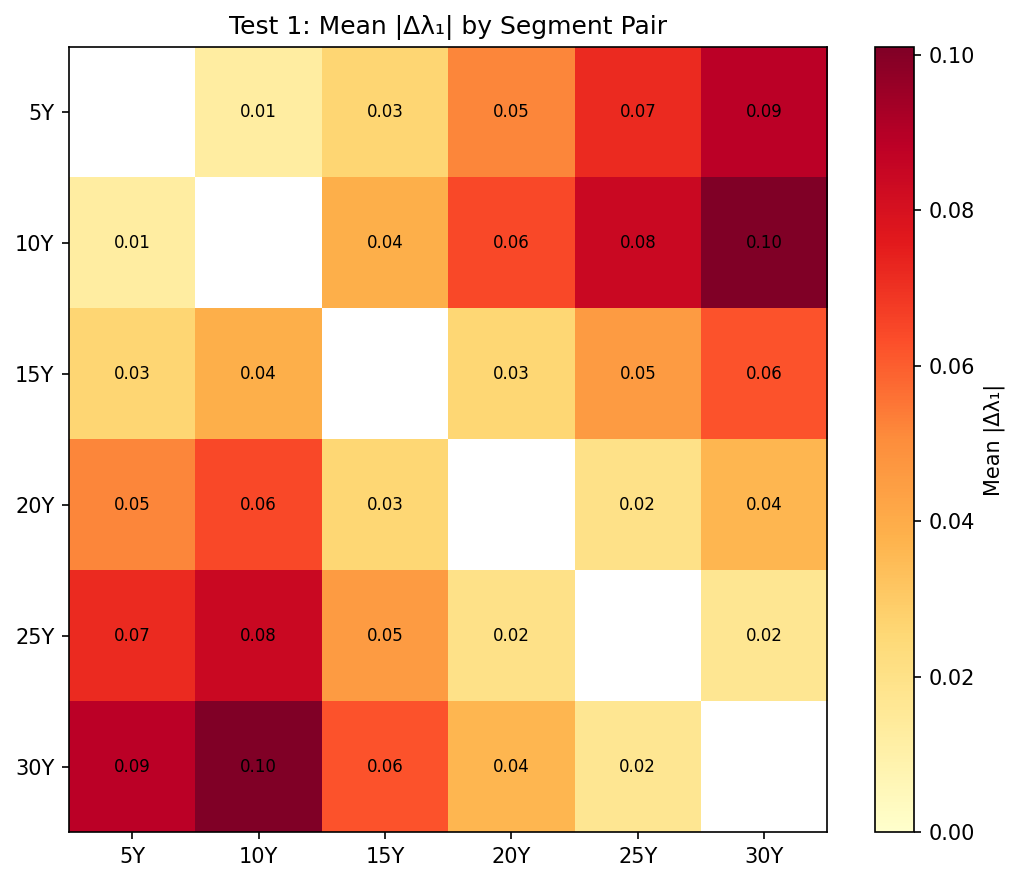
\includegraphics[keepaspectratio,alt={Market Price of Risk Gaps: Heatmap by Segment Pair}]{./figures/test1_lambda_gap_heatmap.png}}
\caption{Market Price of Risk Gaps: Heatmap by Segment Pair}
\end{figure}

\begin{figure}
\centering
\pandocbounded{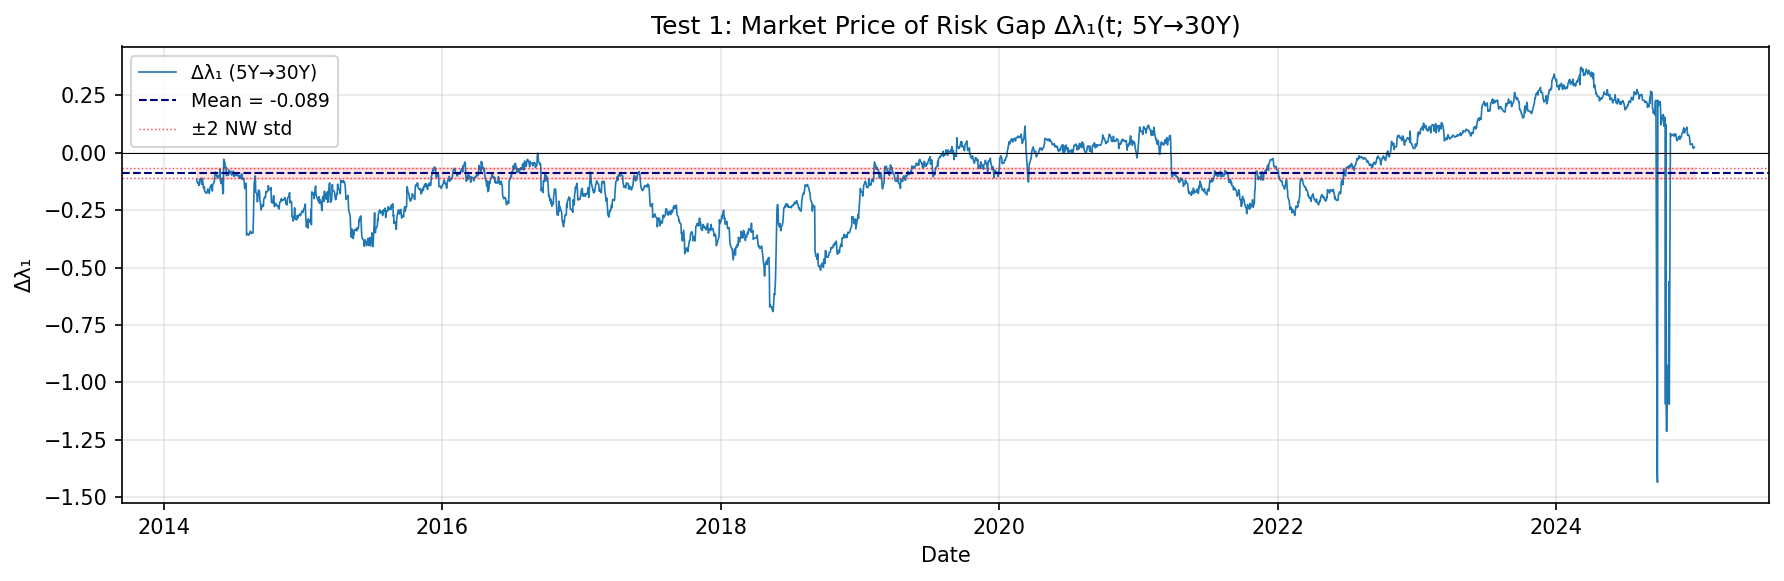
\includegraphics[keepaspectratio,alt={Market Price of Risk Gaps Over Time (5Y vs 30Y)}]{./figures/test1_lambda_gap_timeseries.png}}
\caption{Market Price of Risk Gaps Over Time (5Y vs 30Y)}
\end{figure}

\subsection{4.4 Robustness: Mean-Reversion Bound
Sensitivity}\label{robustness-mean-reversion-bound-sensitivity}

The level factor's mean-reversion parameter \(\kappa_1\) is estimated at
or near its lower bound for segments of 10 years and above on more than
95\% of trading days --- a known identification issue for
near-integrated level factors. To check whether the \(\lambda_1\) gap is
an artefact of this, we re-run with the lower bound raised from 0.01 to
0.05. The results are unchanged: the monotonic pattern and gap
magnitudes are preserved.

\subsection{4.5 Three-Factor Comparison}\label{three-factor-comparison}

If the two-factor \(\lambda\) gaps reflect only model inadequacy, a
three-factor model should reduce them uniformly. The data show something
different.

\textbf{Long-end pairs ($\geq$ 15Y).} The \(\lambda_1\) gaps shrink to near
zero. The curvature factor absorbs the cross-segment discrepancy
entirely. \(R^2\) improves substantially (from 0.84 to 0.94 for the 30Y
segment). For these pairs, the two-factor gap reflects a missing factor,
not a structural feature of the data.

\textbf{Short-vs-long pairs (5Y vs $\geq$ 20Y).} The \(\lambda_1\) gaps do
not shrink --- they widen, from approximately \(-0.09\) to \(-0.25\) to
\(-0.41\). The curvature factor is calibrated with fundamentally
different characteristics across these segments (\(\kappa_3 \approx
0.47\) for 5Y vs.~\(\kappa_3 \approx 1.1\)--\(1.6\) for 15Y+),
suggesting the third factor is doing different work in different parts
of the curve.

This divergent pattern --- gaps vanishing in one region while amplifying
in another --- is the most informative feature of the exercise. A
uniformly misspecified model predicts uniform gap reduction under
enrichment. The data do not show this.

\begin{figure}
\centering
\pandocbounded{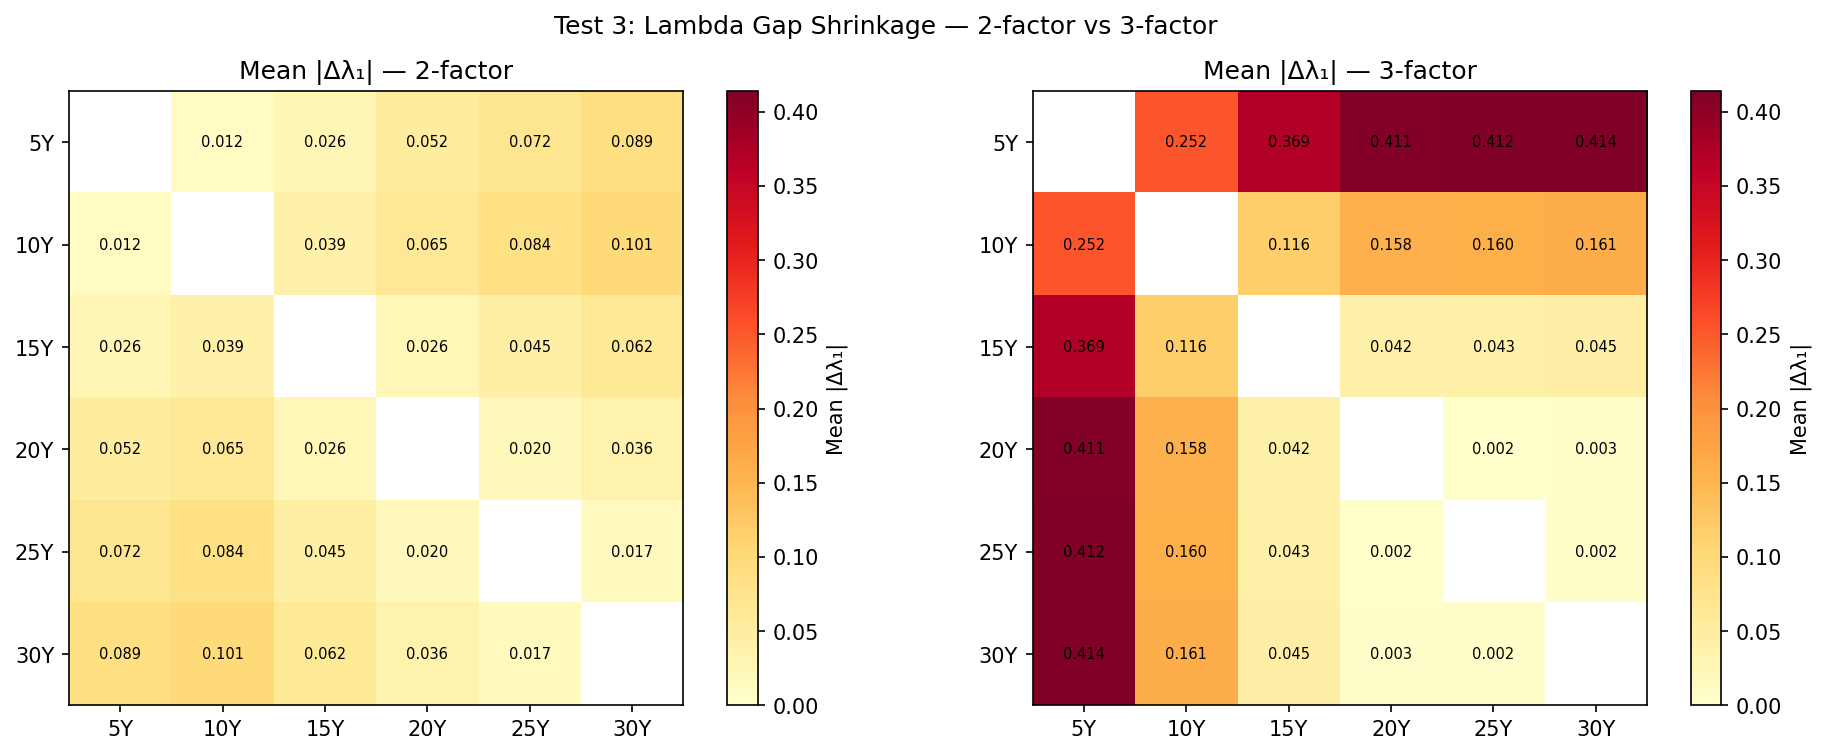
\includegraphics[keepaspectratio,alt={Three-Factor Comparison: Gap Shrinkage by Segment Pair}]{./figures/test3_gap_shrinkage.png}}
\caption{Three-Factor Comparison: Gap Shrinkage by Segment Pair}
\end{figure}

\subsection{4.6 Synthetic Control}\label{synthetic-control}

To assess whether the divergent pattern could arise from the calibration
methodology alone --- even when a single \(Q\) exists by construction
--- we repeat the exercise on synthetic data.

\textbf{Design.} We generate 2,805 daily yield curves from a
three-factor Gaussian HJM with parameters set to the median empirical
estimates from the 30Y segment. By construction, a single \(Q\) exists
and \(\lambda\) is maturity-invariant. We apply the identical
segment-wise calibration procedure.

\textbf{Result.} The synthetic three-factor calibration produces
\(\lambda\) gaps in the range
\(|\Delta\lambda_1| \approx 0.01\)--\(0.09\), uniformly across all
segment pairs. This reflects PCA basis heterogeneity --- each segment's
PCA produces slightly different basis functions, generating apparent
gaps even when true \(\lambda\) is constant. The empirical short-vs-long
gaps (\(0.25\)--\(0.41\)) exceed the same-pair synthetic residuals by
factors of roughly 3--16\(\times\), computed pair by pair across the
5Y-anchor pairs.

Repeating with parameters from the 5Y segment produces a different
synthetic pattern: large gaps with reversed sign
(\(\Delta\lambda_1 \approx +0.14\) to \(+0.22\) across the 5Y-anchor
pairs). Neither DGP reproduces the empirical divergent geometry. The
synthetic exercise is sensitive to DGP specification, which limits its
probative value --- but it does establish that the empirical pattern is
not a generic artefact of segment-wise calibration.

\begin{figure}
\centering
\pandocbounded{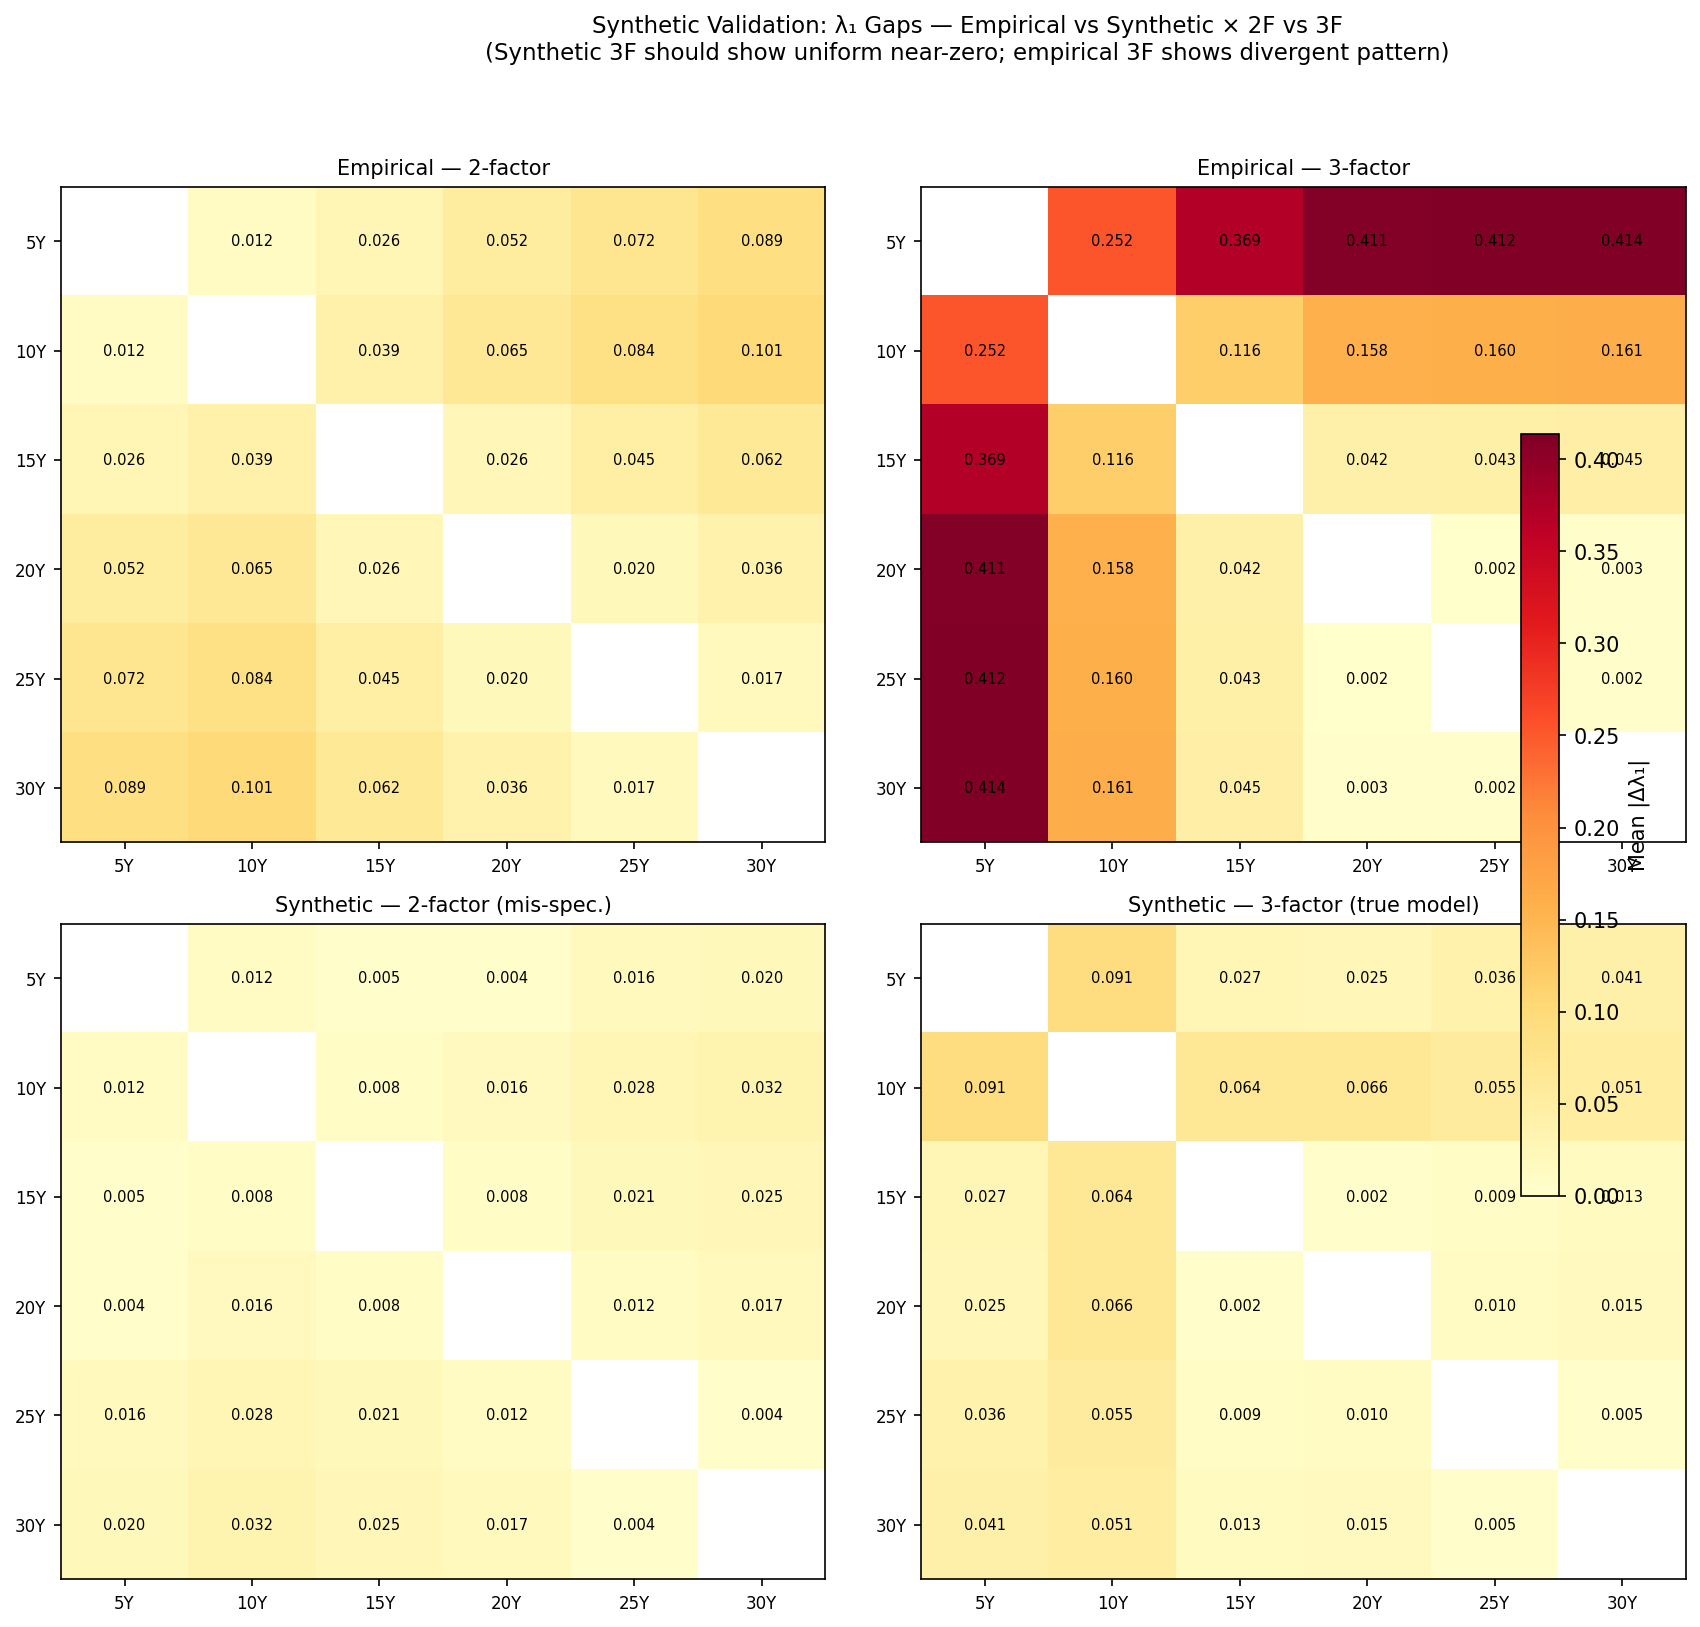
\includegraphics[keepaspectratio,alt={Synthetic vs Empirical: Gap Comparison}]{./figures/synthetic_comparison_heatmap.png}}
\caption{Synthetic vs Empirical: Gap Comparison}
\end{figure}

\subsection{4.7 What the Exercise Shows and Does Not
Show}\label{what-the-exercise-shows-and-does-not-show}

The exercise establishes three things:

First, the forward-measure consistency question has empirical content.
Within the Gaussian HJM class with maturity-independent \(\lambda\),
cross-segment coherence fails in a systematic, monotonic pattern that
standard \(R^2\) diagnostics do not detect.

Second, the three-factor comparison reveals a divergent structure:
long-end gaps are absorbed by an additional factor (model inadequacy),
while short-vs-long gaps amplify (something the model class cannot
reconcile). This divergence is not reproduced by synthetic controls.

Third, the exercise does \emph{not} establish that a single \(Q\) fails
to exist. A single \(Q\) with maturity-dependent \(\lambda(t,T)\) ---
which is precisely what preferred-habitat models produce (Vayanos and
Vila 2021) --- could generate the observed pattern when projected onto a
maturity-independent specification. Distinguishing this from genuine
absence of \(Q\) would require testing within a model class that permits
maturity-dependent \(\lambda\), which we leave to future work.

In particular, because the synthetic control was examined for only two
data-generating parametrisations (30Y- and 5Y-calibrated), and is
sign-sensitive across them, the exercise establishes at most that the
empirical pattern is not a \emph{generic} artefact of segment-wise
calibration --- never that it is irreproducible by \emph{some}
single-\(Q\) model. This ceiling applies to every use of the synthetic
evidence in the paper.

The exercise is a proof of concept for the question, not evidence for
the answer.

\section{5. Directions}\label{directions}

The question formalized in Section 3.3 --- whether pairwise
forward-measure consistency implies the existence of a global \(Q\) ---
is, to our knowledge, open. We identify three directions for
investigation, each requiring expertise beyond the scope of this paper.

\textbf{The mathematical question.} By Lemma 2.4.1 the measure family is
consistent at every finite level; the open content is whether a
numéraire process \(B\) --- equivalently a global \(Q\) --- can be
constructed from a consistent family in continuous time (Section 3.4).
An explicit counterexample --- a consistent family \(\{Q^T\}\) in the
sense of (3.1) admitting no underlying \((Q, B)\) --- would settle the
question negatively and would be the most valuable single contribution.
In finite dimensions with deterministic volatility the problem may be
tractable by functional-analytic methods, with the diagonal
\(r(s) = f(s,s)\) the natural place to seek an obstruction. The
relationship to the no-asymptotic-free-lunch (NAFL) condition of Klein,
Schmidt, and Teichmann (2016) is the most promising connection and is
discussed separately below.

\textbf{Richer model classes and sharper diagnostics.} The empirical
exercise operates within Gaussian HJM with maturity-independent
\(\lambda\). Testing within model classes that permit maturity-dependent
\(\lambda\) \citep{Duffee2002,JoslinSingletonZhu2011} --- or within
non-Gaussian specifications (stochastic volatility, regime-switching)
--- would clarify whether the observed divergent pattern survives or is
absorbed by a richer single-\(Q\) specification. Two refinements would
also sharpen the present diagnostic without changing the model class:
bounding the first-stage (PCA) estimation error --- for instance by
block-bootstrapping the estimation window --- so that the
synthetic-floor margin can be read against first-stage noise; and
partially pinning the direction of the Svensson-smoothing interaction
with segmentation by re-fitting on raw-maturity subsets or perturbing
the input curves. We report the present exercise under explicit caveats
(Section 4) rather than as a calibrated test, and leave these
refinements to future work.

\textbf{The relationship to Klein--Schmidt--Teichmann, and why we do not
claim it.} \citet{KleinSchmidtTeichmann2016} construct a generalized
bank account as a limit of convex combinations of roll-over bonds; by
Section 3.4 our question \emph{is} a numéraire- construction question,
so the two programmes are close, and it is natural to ask whether a
consistent family in the sense of (3.1) implies their
no-asymptotic-free-lunch (NAFL) condition (after which their
construction would supply a generalized \(B\)). We do not claim this
implication, and we state the obstruction precisely. NAFL is a condition
on \emph{trading strategies} in the large financial market generated by
all bonds: it controls sequences of admissible portfolios under a
topology on terminal wealths. Condition (3.1) is a condition on
\emph{measures}: it pins each pairwise density to the
change-of-numéraire form and, by Lemma 2.4.1, glues consistently at
every finite level. Each family member \(Q^{T^*}\) is, by the standing
assumptions of Definition 3.2.1, a measure under which every bond
deflated by \(p(\cdot, T^*)\) is a \emph{true} martingale, and every
other traded asset a local martingale. This resembles KST's
terminal-bond ELMM in form, but differs in scope: KST's ELMM is required
to control the full large-market admissibility closure (sequences of
admissible strategies and their terminal-wealth limits), whereas the
family-derived \(Q^{T^*}\) controls only the finite-dimensional
reweightings that (3.1) encodes and need not regulate that closure.
Condition (3.1) thus says nothing directly about the admissibility class
or the asymptotic closure that NAFL governs. The residual gap is thus
exactly the passage from finite-level measure consistency to a
large-market no-arbitrage condition on strategies; bridging it, to our
understanding, amounts to constructing the numéraire, and we leave it
open. We flag KST as the most likely route to a resolution, not as an
established one.

Separately, the relationship between (BF) and \citeauthor{Herdegen2017}'s (2017)
numéraire-independent no-arbitrage \(\text{NA}^{\text{ni}}\) in
continuous-time bond markets remains open, as noted in Section 2.4.

\section{6. Conclusion}\label{conclusion}

We asked whether the bond market needs a bank account --- whether the
family of T-forward measures \(\{Q^T\}\), built from tradable bonds,
necessarily assembles into a single global risk-neutral measure \(Q\),
or whether \(Q\) is an additional assumption beyond what tradable
instruments can deliver.

In discrete time, the answer is yes: the bank account is constructible
as a self-financing rolling strategy, and a consistent family of forward
measures always exists. In continuous time, the question is open. We
formalized it precisely (Definition 3.2.1), showed that the pairwise
consistency conditions self-propagate (Lemma 2.4.1) with bond-ratio
bubbles excluded by hypothesis, and located the obstruction where it
lives: not in the compatibility of the measure family, nor in a
projective-limit extension, but in the construction of the numéraire
\(B\) (Section 3.4). We stated the precise residual gap to the
large-financial-markets results of \citet{KleinSchmidtTeichmann2016}
without claiming to bridge it, and noted the textbook connection to the
HJM drift condition.

To demonstrate that the question is not vacuous, we conducted a
descriptive empirical exercise. Within the Gaussian HJM class with
maturity-independent market price of risk, cross-segment coherence fails
in a systematic, divergent pattern: long-end discrepancies are absorbed
by an additional curvature factor, while short-vs-long discrepancies
amplify. Synthetic controls indicate this pattern is not a generic
artefact of the calibration methodology. The exercise does not answer
the question --- the observed pattern is consistent with either absence
of a single \(Q\) or inadequacy of the restricted model class --- but it
establishes that the question has empirical teeth.

If this paper contributes anything, it is the question itself. We hope
it may inspire investigation by researchers with the mathematical tools
to resolve it.

\section{Acknowledgments}\label{acknowledgments}

This paper grew out of a puzzle I first encountered during my doctoral
work (Universität Ulm, 2008): why does the standard no-arbitrage theory
rely on a bank account that is not actually traded? The question lay
dormant for eighteen years until the tools existed to revisit it.

The present paper was developed in extended collaboration with Claude
(Anthropic). Claude's contributions included: identifying the original
dissertation result as an algebraic identity rather than an independent
FTAP, which redirected the investigation toward the genuinely open
continuous-time question; surveying and positioning the work relative to
the forward-measure, large-financial-markets, and numéraire-independent
FTAP literatures; iteratively clarifying the question from an intuitive
discomfort into the precise formulation of Definition 3.2.1; designing
the segment-wise calibration approach, the three-factor comparison, and
the synthetic validation; and the scope decision to present this as a
question paper rather than a theorem paper --- matching the contribution
to what the evidence supports. The editorial work, including
structuring, drafting, and responding to reviewer critiques, was
conducted jointly throughout.

Data, code, and reproducible results are available at
https://github.com/shaohui1977/bond-family-na. All errors remain the
author's responsibility.

\section{Appendix A: Proofs for Section
2}\label{appendix-a-proofs-for-section-2}

We prove Proposition 2.3.1. The argument uses three ingredients: the
rolling bond construction makes \(B\) tradable; the classical FTAP
(\citealt{HarrisonPliska1981}) applies; and the numéraire change formula
(\citealt{GemanElKarouiRochet1995}) connects the four conditions.

\textbf{Lemma A.1 (Strategy space equivalence).} The set of terminal
payoffs attainable by self-financing strategies in \(\mathcal{S}\)
coincides with the set attainable in \(\mathcal{S} \cup \{B\}\).

\emph{Proof.} Any strategy holding \(B\) can be replicated by executing
the rolling bond strategy of Proposition 2.2.1, which is self-financing
in \(\mathcal{S}\). \(\quad\square\)

\textbf{Lemma A.2 (Numéraire invariance).} Let \(N\) be a tradable asset
with \(N(t) > 0\), and let \((\varphi, \psi)\) be self-financing with
\(V_0 = 0\). If \(S^j(t)/N(t)\) is a \(Q\)-martingale for all traded
assets \(S^j\), then \(V_t/N(t)\) is a \(Q\)-martingale.

\emph{Proof.} The self-financing condition gives
\(V_t/N(t) - V_{t-1}/N(t-1) = \sum_j \theta^j_t \Delta(S^j/N)_t\), where
\(\theta^j_t\) is predictable and each \(\Delta(S^j/N)_t\) is a
\(Q\)-martingale difference. The sum is therefore a \(Q\)-martingale
difference. \(\quad\square\)

\textbf{Proof of Proposition 2.3.1.}

\((\text{NA}) \iff (\text{EMM})\): By Proposition 2.2.1, \(B\) is the
value of a self-financing strategy with \(B(t) > 0\). By Lemma A.1,
including \(B\) does not enlarge the attainable set. The classical FTAP
(\citealt{HarrisonPliska1981}) gives: \(\text{NA} \iff \exists Q \sim P\)
such that \(S/B\) is a \(Q\)-martingale for all \(S \in \mathcal{S}\).

\((\text{EMM}) \iff (\text{RF})\): For any \(S\) with \(S(t-1) > 0\):
\[E^Q[S(t)/B(t) \mid \mathcal{F}_{t-1}] = S(t-1)/B(t-1)\]
\[\iff E^Q[1 + R_t^S \mid \mathcal{F}_{t-1}] = 1/p(t-1,t)
  = 1 + R_t^{(\text{rf})}\]
\[\iff E^Q[R_t^S \mid \mathcal{F}_{t-1}] = R_t^{(\text{rf})}.\] All
steps are multiplication by positive \(\mathcal{F}_{t-1}\)-measurable
quantities.

\((\text{EMM}) \Rightarrow (\text{BF})\): For each \(T\), define
\[Z^T_t := \frac{p(t,T)}{B(t) \cdot p(0,T)}, \quad
  \frac{dQ^T}{dQ}\bigg|_{\mathcal{F}_t} = Z^T_t.\] Since
\(p(\cdot,T)/B\) is a \(Q\)-martingale, \(Z^T\) is a strictly positive
\(Q\)-martingale with \(Z^T_0 = 1\), so \(Q^T \sim P\). By the abstract
Bayes formula, for \(s \le t \le T\):
\[E^{Q^T}[S(t)/p(t,T) \mid \mathcal{F}_s]
  = \frac{E^Q[Z^T_t \cdot S(t)/p(t,T) \mid \mathcal{F}_s]}{Z^T_s}
  = \frac{E^Q[S(t)/B(t) \mid \mathcal{F}_s] \cdot B(s)}{p(s,T)}
  = \frac{S(s)}{p(s,T)}.\]

\((\text{BF}) \Rightarrow (\text{NA})\): Suppose \(V_0 = 0\),
\(V_N \ge 0\) a.s., \(P(V_N > 0) > 0\). By \((\text{BF})\) with
\(T = N\), \(\exists Q^N \sim P\) such that \(S/p(\cdot,N)\) is a
\(Q^N\)-martingale. By Lemma A.2, \(V_t/p(t,N)\) is a
\(Q^N\)-martingale. Then \(0 = V_0/p(0,N) = E^{Q^N}[V_N/p(N,N)]
= E^{Q^N}[V_N]\). With \(V_N \ge 0\) \(Q^N\)-a.s., this gives
\(V_N = 0\) \(Q^N\)-a.s., hence \(P\)-a.s. Contradiction.
\(\quad\square\)

\textbf{Consistency relation (2.1).} Under \((\text{EMM})\):
\[\frac{dQ^{T_1}}{dQ^{T_2}}\bigg|_{\mathcal{F}_{T_1}}
  = \frac{Z^{T_1}_{T_1}}{Z^{T_2}_{T_1}}
  = \frac{p(T_1,T_1) \cdot p(0,T_2)}{p(0,T_1) \cdot p(T_1,T_2)}
  = \frac{p(0,T_2)}{p(0,T_1) \cdot p(T_1,T_2)}.\] Note that \(B(T_1)\)
cancels. The relation involves only bond prices. \(\quad\square\)


\bibliographystyle{plainnat}
\bibliography{paper}

\end{document}

